\section{基于卷积神经网络的手写数字识别网络设计}
\setchapternum{3}

\subsection{设计原则}

针对 MNIST 图像尺寸小、为单通道灰度图的特点，本文以「参数量小、易于训练、精度高」为设计目标，借鉴堆叠 $3\times3$ 小卷积核加深网络的思想\cite{simonyan2015very}，并引入批量归一化\cite{ioffe2015batch}、ReLU 激活\cite{nair2010rectified}与 Dropout\cite{srivastava2014dropout}以稳定训练、抑制过拟合。

\subsection{网络结构}

本文设计的网络如图\ref{fig:network}所示：输入经四个 $3\times3$ 卷积层（通道数 $32,32,64,64$，均配批量归一化与 ReLU）与两次 $2\times2$ 最大池化逐步提取特征，再由两个全连接层（$3136\rightarrow128\rightarrow10$）完成分类，逐层配置见表\ref{tab:layers}。

\begin{figure}[htb]
\centering
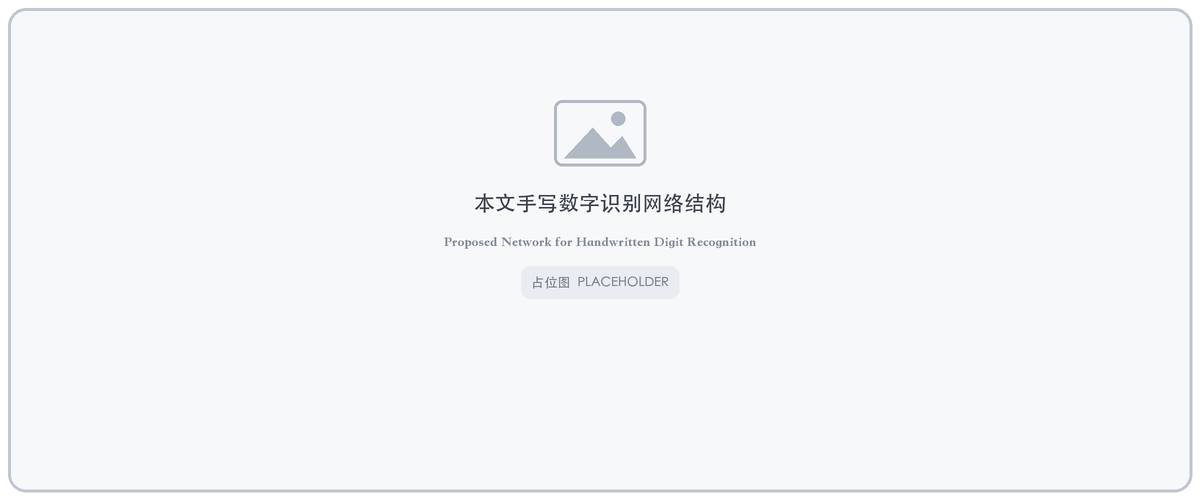
\includegraphics[width=0.95\linewidth]{figures/fig-network-design.png}
\caption{本文手写数字识别网络结构\\Fig.~\thefigure\ Architecture of the proposed network}
\label{fig:network}
\end{figure}

% ===== 三线表示例（booktabs：\toprule / \midrule / \bottomrule；\label 紧跟 \caption）=====
\begin{table}[htbp]
\centering
\caption{本文网络逐层结构配置\\Table~\thetable\ Layer-wise configuration of the proposed network}
\label{tab:layers}
\begin{tabular*}{\linewidth}{@{\extracolsep{\fill}}c c c c}
\toprule
层名称 & 类型 & 输出尺寸 & 卷积核/参数 \\
\midrule
输入 & --- & $1\times28\times28$ & --- \\
Conv1 & 卷积+BN+ReLU & $32\times28\times28$ & $3\times3,\ 32,\ \text{pad}=1$ \\
Conv2 & 卷积+BN+ReLU & $32\times28\times28$ & $3\times3,\ 32,\ \text{pad}=1$ \\
Pool1 & 最大池化 & $32\times14\times14$ & $2\times2$ \\
Conv3 & 卷积+BN+ReLU & $64\times14\times14$ & $3\times3,\ 64,\ \text{pad}=1$ \\
Conv4 & 卷积+BN+ReLU & $64\times14\times14$ & $3\times3,\ 64,\ \text{pad}=1$ \\
Pool2 & 最大池化 & $64\times7\times7$ & $2\times2$ \\
FC1 & 全连接+ReLU+Dropout & $128$ & $3136\times128$ \\
FC2 & 全连接 & $10$ & $128\times10$ \\
输出 & Softmax & $10$ & --- \\
\bottomrule
\end{tabular*}
\end{table}

卷积层参数量由式(\ref{eq:param})估算，据此可得全网参数量约为 $0.47\text{M}$，其中全连接层占绝大部分，卷积层因权值共享而参数很少，整体结构轻量、易于训练。

\begin{equation}
N_{\text{conv}} = K\times K\times C_{\text{in}}\times C_{\text{out}} + C_{\text{out}}
\label{eq:param}
\end{equation}

\subsection{本章小结}

本章给出了本文小型卷积神经网络的设计原则与逐层结构，参数量约 $0.47\text{M}$，为下一章的训练与优化奠定基础。
